\documentclass[twoside,b5paper,10pt]{article}
\usepackage{AUTstyle}

\usepackage{lipsum}                     % Dummytext
\usepackage{xargs}                      % Use more than one optional parameter in a new commands
\usepackage[pdftex,dvipsnames]{xcolor}  % Coloured text etc.

\usepackage[colorinlistoftodos,prependcaption,textsize=tiny]{todonotes}
\newcommandx{\unsure}[2][1=]{\todo[linecolor=red,backgroundcolor=red!25,bordercolor=red,#1]{#2}}
\newcommandx{\change}[2][1=]{\todo[linecolor=blue,backgroundcolor=blue!25,bordercolor=blue,#1]{#2}}
\newcommandx{\info}[2][1=]{\todo[linecolor=OliveGreen,backgroundcolor=OliveGreen!25,bordercolor=OliveGreen,#1]{#2}}
\newcommandx{\improvement}[2][1=]{\todo[linecolor=Plum,backgroundcolor=Plum!25,bordercolor=Plum,#1]{#2}}
\newcommandx{\thiswillnotshow}[2][1=]{\todo[disable,#1]{#2}}
\usepackage{tikz}
\usetikzlibrary{positioning}
\usepackage[siunitx, europeanresistors, americaninductors, voltage shift=0.5]{circuitikz}

\ctikzset{bipoles/thickness=1}
\ctikzset{bipoles/length=0.8cm}
\ctikzset{bipoles/diode/height=.375}
\ctikzset{bipoles/diode/width=.3}
\ctikzset{tripoles/thyristor/height=.8}
\ctikzset{tripoles/thyristor/width=1}
\ctikzset{bipoles/vsourceam/height/.initial=.7}
\ctikzset{bipoles/vsourceam/width/.initial=.7}
\tikzstyle{every node}=[font=\small]
\tikzstyle{every path}=[line width=0.8pt,line cap=round,line join=round]

\title{Comparison of different PMSM motor models}
\author{Dávid Kiss}

\institution{Department of Automation and Applied Informatics \\
Budapest University of Technology and Economics}

\email{david.kiss@aut.bme.hu}

\headerTitle{Comparison of different PMSM motor models \dots}
\headerAuthor{Dávid Kiss}


\begin{document}
\makeAutStyleTitle

\begin{abstract}
Electrical drive simulation is one of the key areas of the emerging trends in power electronics. There are many off-the-shelf solutions available on the market, even engineering tools, like Matlab/Simulink developed it's own solution for the problem in the Simscape Electrical toolbox. There are claims, the solutions from different suppliers are applicable for on-line (real-time) simulation, which is important in HIL\footnote{Hardware-in-the-Loop} and P-HIL\footnote{Power Hardeare-in-the-Loop} environments. This Paper focuses on the validation of the PMSM model provided by MATLAB/Simulink.
\end{abstract}


\begin{keywords}
Simulation; PMSM; MATLAB; Real-Time AACS Workshop; (list of $5$-$7$ keywords in this
format)
\end{keywords}

\listoftodos

\section{Introduction}
\label{sec:Introdu}

\todo[inline]{Nincs még kész.}

\section{Mathematical model of a PMSM Machine}
\label{sec:matPMSM}

The Automotive industry always played a key role in innovation and always pioneered with new and emerging technologies. The situation is no different in the case of electrification nowadays. Electrical motors are the core element of modern hybrid (HEV) and Battery Electric Vehicle's (BEV) drivetrains. Volume and mass is a very limiting factor, especially in the case of BEV vehicles, because the saved mass and volume provides more space for the battery itself, providing higher range for the vehicle. Because of these reasons, 3-phase induction (IM\footnote{Induction Machine}) and PMSM\footnote{Permanent Magnet Synchronous Machine} machines are commonly used in traction (and other actuation) systems in the automotive industry. The difference between these two type of electrical machines is the source of the magnetic flux inside. In the case of the IM the magnetic field has to come from external excitation, in the PMSM machine, as the name suggests, the magnetic field is generated by the built-in permanent magnets. PMSM machines are especially superior in power density, however their drawback is the necessity of complex control algorithms and the expensive magnetic material.

\info[inline]{Itt még be kell hivatkozni Veszprémi könyvét meg írni arról, hogy miért király a PMSM!}


This paper details the mathematical description of the PMSM due to it's simplicity, with the following assumptions:
\begin{itemize}
  \item The machine is symmetrical ($L_d = L_q$)
  \item The stator winding are in star connection
  \item Losses are neglected (Ventillation, internal friction, iron losses)
  \item Coil inductances and resistances are constant
\end{itemize}

\begin{figure}[htb]
\begingroup
\tikzset{}
 \centerline{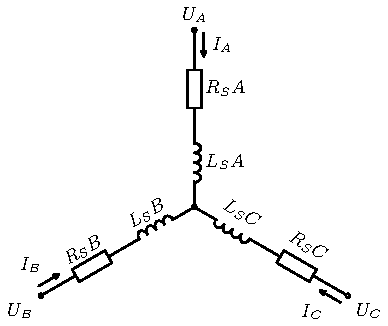
\includegraphics[width=.35\columnwidth]{.//Figure/threephase_winding.pdf}}
 \endgroup
 \caption{The equvalent circuit of a 3-phase motor winding}
 \label{fig:threephase_winding}
\end{figure}

\begin{gather}
\label{eq:clark}
    \begin{bmatrix}
    \alpha \\ \beta \\ 0
    \end{bmatrix}
    =
    \frac{2}{3}
    \begin{bmatrix}
    1 & -\frac{1}{2} & -\frac{1}{2} \\[0.5em]
    0 & \frac{\sqrt{3}}{2} & -\frac{\sqrt{3}}{2} \\[0.5em]
    \frac{1}{2} & \frac{1}{2} & \frac{1}{2}
    \end{bmatrix}
    \begin{bmatrix}
    a \\ b \\ c
    \end{bmatrix}
\end{gather}
\begin{gather}
\label{eq:inv_clark}
    \begin{bmatrix}
     a \\ b \\ c
    \end{bmatrix}
    =
    \begin{bmatrix}
    1            & 0                  & 1             \\[0.5em]
    -\frac{1}{2} & \frac{\sqrt{3}}{2} & 1             \\[0.5em]
    -\frac{1}{2} & -\frac{\sqrt{3}}{2}& 1
    \end{bmatrix}
    \begin{bmatrix}
     \alpha \\ \beta \\ 0
    \end{bmatrix}
\end{gather}
\begin{gather}
\label{eq:park}
    \begin{bmatrix}
    d\\ q \\ 0
    \end{bmatrix}
    =
    \frac{2}{3}
    \begin{bmatrix}
    sin(\theta) & sin(\theta-\frac{2\pi}{3}) & sin(\theta+\frac{2\pi}{3}) \\[0.5em]
    cos(\theta) & cos(\theta-\frac{2\pi}{3}) & cos(\theta+\frac{2\pi}{3}) \\[0.5em]
    \frac{1}{2} & \frac{1}{2}                & \frac{1}{2}
    \end{bmatrix}
    \begin{bmatrix}
    a \\ b \\ c
    \end{bmatrix}
\end{gather}
\begin{gather}
\label{eq:inv_park}
    \begin{bmatrix}
    a \\ b \\ c
    \end{bmatrix}
    =
    \begin{bmatrix}
    sin(\theta)                & cos(\theta)                & 1                   \\[0.5em]
    sin(\theta-\frac{2\pi}{3}) & cos(\theta-\frac{2\pi}{3}) & 1                   \\[0.5em]
    sin(\theta+\frac{2\pi}{3}) & cos(\theta+\frac{2\pi}{3}) & 1
    \end{bmatrix}
    \begin{bmatrix}
    d\\ q \\ 0
    \end{bmatrix}
\end{gather}



\begin{align} 
\label{eq:dc_dt}
u(t) &= i(t) + L\frac{di(t)}{dt} + u_b(t) \\ 
u_b(t) &= k\Phi{}\omega{}(t) \\
m(t) - m_t(t) &= \Theta{}\frac{d\omega{}(t)}{dt} \\
m(t) &= k\Phi{}i(t) \\
\omega{}(t) &= \frac{d\alpha(t)}{dt}
\end{align}

\begin{align*} 
u(s) &= Ti(s) + Lsi(s) + u_b(s) \\ 
u_b(s) &= k\Phi{}\omega{}(s) \\
m(s) - m_t(s) &= \Theta{}s\omega{}(s) \\
m(s) &= k\Phi{}i(s) \\
\omega{}(t) &= s\alpha(s)
\end{align*}

 \begin{figure}[h]
        \centering
%%----start of first subfigure----
        \subfloat[Interior magnets]{
            \label{subfig:one} %% label for first subfigure
            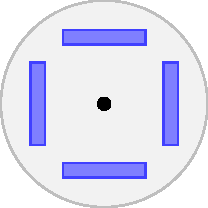
\includegraphics[width=0.2\linewidth]{Figure/motor_interior.pdf}}
        \hspace{0.02\linewidth}
%%----start of second subfigure----
        \subfloat[Surface mounted magnets]{
            \label{subfig:two} %% label for second subfigure
            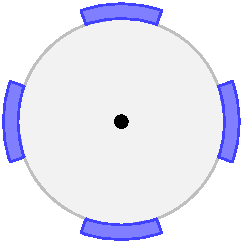
\includegraphics[width=0.2\linewidth]{Figure/motor_exterior.pdf}}
        \caption{PMSM Motor types}
        \label{fig:mot_sailient_non} %% label for entire figure
\end{figure}

 \begin{figure}[h]
        \centering
%%----start of first subfigure----
        \subfloat[Stator Reference frame]{
            \label{subfig:one} %% label for first subfigure
            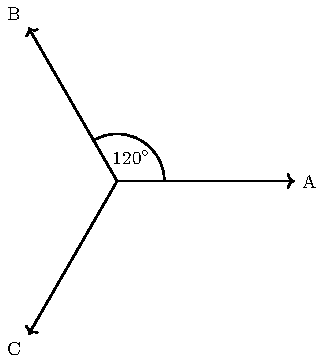
\includegraphics[width=0.3\linewidth]{Figure/coord_abc.pdf}}
        \hspace{0.02\linewidth}
%%----start of second subfigure----
        \subfloat[$\alpha\beta$ and $dq$ Reference frame]{
            \label{subfig:two} %% label for second subfigure
            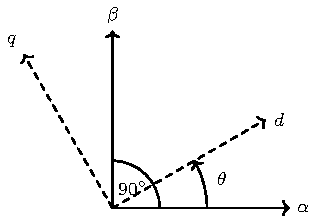
\includegraphics[width=0.3\linewidth]{Figure/coord_alpha_dq.pdf}}
        \caption{Different reference frames}
        \label{fig:bme} %% label for entire figure
\end{figure}


\section{Bibliography}
\label{sec:bib}

You have to use the \verb|\makeAutBib| command for your
bibliography. The input parameter of the command is the comma
separated list of bib files without the extension. You can also find
a sample bib file on the Workshop's web site where also the style
file and this sample \LaTeX \ template are provided. You can cite
any of the entries of the bib files for example ~\cite{ han00mining}
or ~\cite{burdick01mafia}. The advantage of using bib files is that
only those bibliographies will appear in the References section that
are cited in the text \cite{proba}.

If you have any question related to writing your \LaTeX \ paper
please contact the chair of the conference(e-mail: aacs@aut.bme.hu).

You can submit your paper via the web page of the conference. The
submission of the papers will be opened soon.

\section*{Acknowledgments}
 { \small The author would like to express his thanks to István Vajk~\footnote{Please mention the name of your advisor in the
Acknowledgements section. } for his support as a scientific advisor.
This work has been supported by the \dots \footnote{Please mention
the institution or organization that has supported your research
work.} }

\makeAutBib{reni,itemsetmining}

\end{document}
